\documentclass[11pt]{article}

\usepackage[a4paper,margin=2.7cm]{geometry}
\usepackage{amsmath,amssymb,bm}
\usepackage{graphicx}
\usepackage{booktabs}
\usepackage{caption}
\usepackage{subcaption}
\usepackage{tikz}
\usepackage[colorlinks=true,linkcolor=blue,citecolor=blue,urlcolor=blue]{hyperref}
\usetikzlibrary{positioning,fit,backgrounds,arrows.meta}

\newcommand{\vA}{v_{A}}
\newcommand{\vB}{v_{B}}
\newcommand{\DA}{D_A}
\newcommand{\DB}{D_B}
\newcommand{\DAB}{D_{AB}}
\newcommand{\TODO}[1]{\textit{[#1]}}

\title{Interaction-specific structure in coupled protein families:\\
a modular, frozen-and-added Restricted Boltzmann Machine}
\author{}
\date{}

\begin{document}
\maketitle

\begin{abstract}
Many biological systems are organised not as single homogeneous
statistical ensembles but as families of interacting subsystems:
physically or functionally coupled protein families that have coevolved
under a shared constraint. We are interested in modelling such
interacting family pairs generatively, in the regime that is actually
relevant for most biological interactions of interest: single-family
sequence data are abundant, while paired, interaction-labelled data are
scarce. We propose a modular Restricted Boltzmann Machine (RBM)
architecture that exploits this asymmetry directly. Two RBMs are first
pretrained independently on the abundant single-family data, until each
reproduces its own family's statistics; their parameters are then frozen
inside a larger, paired model, and a small block of newly added hidden
units, connected to the full joint visible layer, is left free to absorb
whatever the two frozen, independent models fail to explain -- by
construction, only genuine inter-family structure. This isolates a
minimal, identifiable channel for interaction-specific information, and
makes the paired-training stage cheap in the one resource that is
actually scarce. We validate this construction on a two-family Ising/Potts spin system with
a known, hidden ground-truth coupling matrix, used as a controlled test
case and confirmed stable across independent random realisations
(Appendix~\ref{app:ising}), and then apply the identical architecture and
training recipe, unchanged, to two real pairs of coevolving Pfam protein
domains that share a common family (Section~\ref{sec:protein}). In both
protein systems, the added units recover cross-family correlation
structure that lies far above an independent-model null, though further
from the finite-sample ceiling than in the controlled case; an
independent, energy-based test correctly recovers the true interaction
partner among candidate paralogs, well above chance, in both systems; and
clamped conditional generation reproduces true-partner-specific structure
beyond both a wrong-partner control and a naive consensus baseline. Taken
together, these results support the central hypothesis -- that
interaction-specific structure can be attributed to a small, cheaply
trainable channel added on top of frozen, independently pretrained models
-- while also indicating that real coevolutionary signal is harder to
recover in full than the sparse, synthetic coupling of the controlled test
case.
\end{abstract}

\section{Motivation}
\label{sec:motivation}

Many complex systems of interest in statistical physics are not single
homogeneous systems but collections of subsystems that interact weakly
with one another: coupled spin lattices, interacting populations of
neurons, or -- the case that concerns us here -- correlated families of
biological sequences. Protein domain families evolve largely
independently, subject to their own internal structural and functional
constraints, but pairs of families that physically interact or act in the
same pathway (a receptor and its ligand, a kinase and its substrate, two
subunits of the same complex) are additionally constrained by the
requirement of \emph{mutual} compatibility: an amino-acid substitution on
one side of an interaction interface is only tolerated if compensated,
directly or diffusely, on the other side. This coevolutionary signal is
exactly analogous to a genuine physical coupling between two otherwise
weakly-interacting statistical-mechanical subsystems, and inferring it
from sequence data alone is a classic, still largely open, inverse
problem.

What makes this problem distinctive in practice is a strong data
asymmetry. Single-family sequence databases are enormous and growing:
hundreds of thousands of natural sequences are available for many
individual Pfam domains. Data in which two specific, interacting family
members are \emph{paired} -- known to co-occur in the same functional
complex or operon -- are comparatively scarce, since establishing a
correct pairing typically requires either genomic proximity heuristics,
experimental validation, or a species with a small enough paralog count
that pairing is unambiguous. Any inference method that requires large
amounts of paired data to work is, in this sense, solving the wrong
problem: the practically relevant question is how much can be learned
about the interaction itself from the much smaller paired data set,
\emph{given that the bulk of statistical structure -- everything about
each family in isolation -- can already be learned essentially for free}
from the abundant unpaired data.

This project's central bet is to take that asymmetry seriously at the
level of model architecture, not just training-set size. An RBM is
already a natural generative model for a single sequence family: its
hidden layer acts as an auxiliary field mediating effective, non-pairwise
interactions among the visible (sequence) units once marginalised out, in
the same spirit as a Hubbard--Stratonovich decoupling of a many-body
interaction, which is what makes it more expressive than a purely
pairwise (Potts/DCA-type) model while remaining tractable. Our proposal
is to pretrain one such RBM per family on the abundant single-family
data, \emph{freeze} its parameters, and then ask whether a small,
newly-added block of hidden units, connected to the full joint (paired)
visible layer and trained only on the scarce paired data, is sufficient
to capture the interaction-specific structure that a pair of independent,
frozen models cannot represent by construction. If it is, the paired
data requirement for learning interaction specificity is reduced to
whatever is needed to fit a small number of new parameters, rather than
an entire joint model.

This sits at the intersection of two questions, one practical and one
more fundamental to representation learning:
\begin{itemize}
\item \textbf{Practical.} Can we build a generative model of an
interacting protein family pair that is trainable with a realistically
small paired data set, while still producing high-quality conditional and
joint samples -- ultimately, given a sequence from family $A$, a
plausible, specific partner from family $B$?
\item \textbf{Fundamental.} What does a model learn, and how efficiently,
when a small, structurally isolated subset of its parameters is forced to
encode exactly the information that a set of frozen, pretrained
components cannot -- an explicit, testable instance of forcing a
representation to specialise?
\end{itemize}

\section{The scientific question}
\label{sec:question}

We restate the motivation of Section~\ref{sec:motivation} as a precise,
falsifiable question, so that the validation strategy of
Section~\ref{sec:validation} can be judged against it directly.

\textbf{Setting.} Two protein families $A$ and $B$, with $N_A$ and $N_B$
alignment columns respectively over a $q$-letter alphabet (amino acids
plus gap, $q=21$, for real sequences; a $q=2$ Ising spin for the
controlled test case of Appendix~\ref{app:ising}). We have access to
\begin{itemize}
\item abundant single-family data sets $\DA$, $\DB$ (unpaired sequences
of each family separately, $|\DA|,|\DB|$ large), and
\item a much smaller paired data set $\DAB$ of sequences known, by some
external criterion, to interact (e.g.\ genomic co-occurrence),
$|\DAB|\ll|\DA|,|\DB|$.
\end{itemize}

\textbf{Goal.} Learn a joint generative model $p_\theta(v_A,v_B)$ such
that:
\begin{enumerate}
\item[(a)] the marginals $p_\theta(v_A)$ and $p_\theta(v_B)$ are as
faithful to $\DA$ and $\DB$ as models trained directly and exclusively on
$\DA$, $\DB$ -- pairing must not degrade what is already learnable from
the abundant single-family data;
\item[(b)] the joint distribution captures genuine inter-family
structure -- residue-residue covariation between sites of $A$ and sites
of $B$ that reflects a true interaction constraint -- learned efficiently
from the small $\DAB$.
\end{enumerate}

\textbf{Falsifiable success criteria.} Because there is generally no
ground-truth coupling to compare against for real protein families, we
adopt the same triangulation used throughout statistical inference from
finite samples: any recovered signal must be judged relative to a
\emph{null} (what a model with no shared structure at all would produce)
and a \emph{ceiling} (what the finite paired sample itself can support,
irrespective of the model). Concretely, the architecture of
Section~\ref{sec:architecture} is judged to be working if the
inter-family structure recovered by the trained paired model
\begin{itemize}
\item lies far above the level recovered by two independently trained,
uncoupled models sharing no hidden units at all (the \emph{null}), and
\item approaches, as closely as the amount of paired training data
allows, the level of agreement between two independent finite samples of
the true interacting distribution (the \emph{ceiling}) --
\end{itemize}
while simultaneously satisfying (a): the frozen single-family blocks must
still reproduce their own family's statistics at equilibrium. A result in
which the paired model sits at the null (no interaction signal learned)
or in which pairing measurably corrupts single-family statistics would
falsify the construction as currently designed.

\section{Architecture: a modular, frozen-and-added RBM}
\label{sec:architecture}

An RBM is a pairwise energy-based model on a bipartite graph of visible
units $\bm{v}$ and hidden units $\bm{h}$, with joint Boltzmann weight
\begin{equation}
p(\bm{v},\bm{h}) \propto \exp\!\big[-E(\bm{v},\bm{h})\big], \qquad
E(\bm{v},\bm{h}) = -\bm{v}^\top W \bm{h} - a(\bm{v}) - b(\bm{h}) \, ,
\label{eq:rbm-energy}
\end{equation}
where $W$ is a visible--hidden weight matrix and $a$, $b$ are
layer-specific potentials. The absence of visible--visible and
hidden--hidden couplings makes both conditionals, $p(\bm{h}\mid\bm{v})$
and $p(\bm{v}\mid\bm{h})$, factorised and hence efficiently sampled, while
the marginalised hidden layer still mediates effective, non-pairwise
interactions among the visible units (Section~\ref{sec:motivation}). The
visible layer is Potts-encoded ($q$-state categorical units, one-hot,
sampled through a Gumbel-softmax relaxation), paired with hidden units of
the dReLU family (continuous, rectified, with both positive- and
negative-going branches), which generalise the Bernoulli hidden unit to a
richer response function; the same construction specialises to $q=2$,
Bernoulli-hidden ``binary'' RBMs as a limiting case, used in
Appendix~\ref{app:ising} for direct comparison. Both variants are wrapped
with an online re-standardisation of the visible and hidden layers and,
for the Potts layer, a zero-sum gauge fixing of the categorical weights.

\subsection{The paired construction}
\label{sec:paired-construction}

Given two RBMs pretrained independently on $\DA$ and $\DB$
(Section~\ref{sec:training}), we build a single, larger \emph{paired}
model as follows (Fig.~\ref{fig:architecture}):

\begin{enumerate}
\item The visible layer of the paired model is the concatenation of the
two families' visible layers, $v=(v_A,v_B)$, $N_A+N_B$ sites in total.
\item The hidden layer is the concatenation of three blocks: the $n_A$
hidden units of the independently trained $A$-model, the $n_B$ hidden
units of the independently trained $B$-model, and $n_{\mathrm{add}}$
newly \emph{added} hidden units with no prior identity.
\item The weight blocks $W_{v_A h_A}$ and $W_{v_B h_B}$ are initialised
from the independently trained models and then \emph{frozen}: after
every gradient step of the paired model's training, these blocks (and the
corresponding visible/hidden biases) are reset to their pretrained
reference values, discarding whatever update the optimiser proposed for
them. This projection-based freezing is equivalent in effect to excluding
these parameters from the gradient, but is implemented as a reset for
convenience, and is checked at every logged step against drift.
\item The cross blocks $W_{v_B h_A}$ and $W_{v_A h_B}$ are pinned at
exactly zero throughout training: the private hidden units of one family
have, by construction, no direct view of the other family's sequence.
\item The only parameters left genuinely free to adapt under gradient
ascent are the weight blocks $W_{v_A h_{\mathrm{add}}}$ and
$W_{v_B h_{\mathrm{add}}}$ connecting the added hidden units to the
\emph{full} joint visible layer, together with the added units' own
biases.
\end{enumerate}

By construction, any cross-family statistical dependence that the paired
model is capable of representing must flow through the added units: they
are the sole channel connecting $A$ and $B$. If they learn nothing, the
paired model is exactly equivalent, in its predictions, to two
independent, non-interacting RBMs -- the null model of
Section~\ref{sec:question}. If they learn something, it can only be
inter-family structure, since every other parameter is already fixed to
reproduce single-family statistics as well as the private models do. This
is the sense in which the construction isolates a minimal, identifiable
channel for interaction-specific information, and directly operationalises
the fundamental question of Section~\ref{sec:motivation}: what is learned
when only this channel is left free to specialise.

\begin{figure}[htb]
\centering
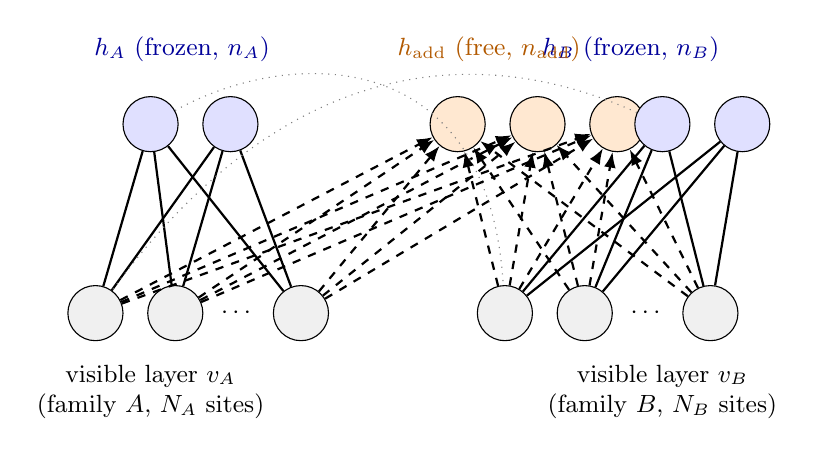
\begin{tikzpicture}[
  node distance=10mm,
  unit/.style={circle, draw, minimum size=7mm, inner sep=0pt},
  frozen/.style={unit, fill=blue!12},
  addedu/.style={unit, fill=orange!18},
  visu/.style={unit, fill=gray!12},
  frozenedge/.style={draw, thick},
  freeedge/.style={draw, thick, dashed, -{Latex[length=2mm]}},
  zeroedge/.style={draw, thin, dotted, gray},
  font=\small
]

  \node[visu] (vA1) at (0,0) {};
  \node[visu] (vA2) [right=3mm of vA1] {};
  \node (vAdots) [right=1mm of vA2] {$\cdots$};
  \node[visu] (vA3) [right=1mm of vAdots] {};
  \node[visu] (vB1) at (5.2,0) {};
  \node[visu] (vB2) [right=3mm of vB1] {};
  \node (vBdots) [right=1mm of vB2] {$\cdots$};
  \node[visu] (vB3) [right=1mm of vBdots] {};

  \node[frozen] (hA1) at (0.7,2.4) {};
  \node[frozen] (hA2) [right=3mm of hA1] {};
  \node[addedu] (hadd1) at (4.6,2.4) {};
  \node[addedu] (hadd2) [right=3mm of hadd1] {};
  \node[addedu] (hadd3) [right=3mm of hadd2] {};
  \node[frozen] (hB1) at (7.2,2.4) {};
  \node[frozen] (hB2) [right=3mm of hB1] {};

  \foreach \h in {hA1,hA2}
    \foreach \v in {vA1,vA2,vA3}
      \draw[frozenedge] (\v) -- (\h);
  \foreach \h in {hB1,hB2}
    \foreach \v in {vB1,vB2,vB3}
      \draw[frozenedge] (\v) -- (\h);

  \foreach \h in {hadd1,hadd2,hadd3}
    \foreach \v in {vA1,vA2,vA3,vB1,vB2,vB3}
      \draw[freeedge] (\v) -- (\h);

  \draw[zeroedge] (hA1) .. controls (2.5,3.4) and (5.0,3.4) .. (vB1);
  \draw[zeroedge] (hB1) .. controls (5.0,3.4) and (2.5,3.4) .. (vA1);

  \node[align=center] at (0.7,-1.0) {visible layer $\vA$\\(family $A$, $N_A$ sites)};
  \node[align=center] at (7.2,-1.0) {visible layer $\vB$\\(family $B$, $N_B$ sites)};
  \node[align=center,text=blue!60!black] at (1.1,3.35) {$h_A$ (frozen, $n_A$)};
  \node[align=center,text=blue!60!black] at (6.8,3.35) {$h_B$ (frozen, $n_B$)};
  \node[align=center,text=orange!70!black] at (5.0,3.35) {$h_{\mathrm{add}}$ (free, $n_{\mathrm{add}}$)};

\end{tikzpicture}
\caption{Architecture of the paired RBM. Solid edges: private
$A$--$A$ and $B$--$B$ weight blocks, pretrained independently and reset
to their reference values after every gradient step (``frozen''). Dotted
grey edges: the cross blocks $h_A$--$\vB$ and $h_B$--$\vA$, permanently
pinned at zero. Dashed orange edges: the only free parameters in the
paired model, connecting the $n_{\mathrm{add}}$ added hidden units to the
full, joint visible layer.}
\label{fig:architecture}
\end{figure}

\section{Training curriculum}
\label{sec:training}

Maximum-likelihood training of an RBM requires the gradient of the
log-likelihood, which contains a data-averaged and a model-averaged term;
the latter is estimated by Persistent Contrastive Divergence (PCD), i.e.\
a set of Monte Carlo chains that are carried over and advanced by a fixed
number of sweeps between successive gradient steps, rather than
reinitialised at every step. Training throughout uses PCD with the Adam
adaptive step-size rule.

Training proceeds in two stages, deliberately separated so that the
second, expensive-data stage is as cheap as possible in the number of
free parameters and gradient steps required:

\begin{enumerate}
\item \textbf{Pretraining (abundant data).} Each family's private RBM is
trained independently on its own single-family data set ($\DA$ or $\DB$)
until its own held-out pseudolikelihood and moment-matching diagnostics
(Section~\ref{sec:validation}) indicate convergence, with no reference at
all to the other family or to any paired data.
\item \textbf{Pair-training (scarce data).} The two pretrained models are
assembled into the paired architecture of
Section~\ref{sec:paired-construction} and the added block is trained,
with the private blocks frozen, on the paired data set $\DAB$ only. Since
the number of free parameters at this stage is a small fraction of the
full paired model's parameter count, and the private blocks already
provide a correct single-family generative prior, this stage is expected
to require substantially less data and substantially fewer gradient steps
to converge than training the equivalent full joint model from scratch --
this expectation is itself part of what Section~\ref{sec:validation} is
designed to test.
\end{enumerate}

\section{Validation methodology}
\label{sec:validation}

We use two complementary levels of diagnostic, applied identically to the
controlled test case (Appendix~\ref{app:ising}) and to the protein system
(Section~\ref{sec:protein}).

\paragraph{Training-time diagnostics.} During pair-training we
periodically compare, along the same short persistent Monte Carlo chains
used for the gradient estimate, data-averaged and model-averaged
statistics: visible--hidden correlations $\langle v_i h_\mu\rangle$
(``$vh$-check''), visible--visible correlations $\langle v_i v_j\rangle$
(``$vv$-check''), the inter-family correlation specifically (``$ab$-check''),
hidden-unit firing rates from actual samples rather than mean-field values
(to catch collapsed, always-on/off units that moment-based checks alone
can miss), the weight norm of the added units' incoming visible weights
(to check they are acquiring receptive-field structure at all), and the
raw free-gradient norm on the added block (to distinguish converged from
merely stuck). A dedicated freeze check verifies, at every logged step,
that the nominally frozen blocks have in fact not drifted from their
reference values. These are cheap, on-line diagnostics of convergence,
not a substitute for a proper equilibrium test, since the persistent
chains used during training are advanced by only a handful of sweeps per
step and are not guaranteed to be equilibrated.

\paragraph{Equilibrium validation.} The decisive test is performed
\emph{after} training, on the frozen, converged model: a large number of
independent Gibbs chains are run from random initial conditions for long
enough that a free-energy burn-in diagnostic shows a stationary plateau
(state-space size dependent -- see the equilibration caveat below), and
the resulting equilibrium samples are used to estimate the model's
cross-family correlation structure. This is compared against the best
available truth proxy -- the known coupling matrix in the controlled test
case, a held-out paired split in the protein case -- via (i) the fraction
of the strongest true/reference couplings that are also among the
strongest correlations recovered by the model (``top-$K$ overlap''), and
(ii) the correlation between the full recovered structure and the
reference. Both quantities are also computed for the finite paired
training sample itself (the \emph{ceiling}, Section~\ref{sec:question})
and for the independent, uncoupled-model \emph{null}. The same
equilibrium samples are further decomposed by hidden block (frozen vs.\
added, mirroring Fig.~\ref{fig:architecture}) to check that pairing has
not corrupted the frozen blocks' agreement with single-family data, and
by intra-family correlation (``family preservation'') to check that
recovering cross-family signal has not come at the cost of each family's
own statistics.

\paragraph{An equilibration caveat.} The free-energy burn-in diagnostic is
not a formality: the number of Gibbs sweeps needed to reach a stationary
distribution grows sharply with the size of the state space, and a
$q^{N}$-state categorical system with $q=21$ and $N\sim100$--$200$ sites
mixes far more slowly under single-site Gibbs updates than a $q=2$,
$N=30$-spin toy system. Equilibrium comparisons drawn from chains that
have not visibly plateaued should be read as a lower, one-sided bound
rather than a converged estimate, and this is checked explicitly, not
assumed, for every system studied (see Appendix~\ref{app:ising} for the
controlled case and Section~\ref{sec:protein} for the protein case).

\section{Application: real interacting protein-domain pairs}
\label{sec:protein}

We apply the architecture and training curriculum of
Sections~\ref{sec:architecture}--\ref{sec:training}, unchanged, to two
real pairs of coevolving Pfam domains that share a common family $A$,
PF00072 (response regulator receiver): a standard two-component
signal-transduction pairing with PF00512 (histidine kinase), and a
chemotaxis-pathway pairing with PF01339 (CheB methylesterase). Testing
the construction on two independent family-$B$ partners, with a common
family-$A$ pretrained model family, lets us ask whether the recovered
interaction signal is a property of the architecture or an accident of
one particular pair. Family $A$ is the first $111$ alignment columns in
both data sets; family $B$ is the remaining columns, $66$ for PF00512 and
$174$ for PF01339. Visible units are one-hot, $q=21$-state Potts
variables (the $20$ amino acids plus the alignment gap symbol).
\texttt{PF00072\_PF00512\_paired.fasta} contains $77\,880$ sequence pairs;
\texttt{PF00072\_PF01339\_paired.faa} contains $27\,548$. In both cases
sequences are shuffled and split into training, validation and held-out
sets, the held-out split serving as the truth proxy of
Section~\ref{sec:validation} since no ground-truth coupling matrix exists
for real sequence data.

\subsection{Setup}

The private RBMs use $150$ (family $A$) and $100$ (family $B$) hidden
units, pretrained on the single-family alignment columns with the
PCD/Adam recipe of Section~\ref{sec:training}. The paired model adds
$n_{\mathrm{add}}=20$ free hidden units on top of the two frozen private
blocks, connected to the full joint visible layer ($177$ sites for
PF00512, $285$ for PF01339), and is pair-trained on $\DAB$ with the
identical freeze-and-reset mechanism of
Section~\ref{sec:paired-construction}. Cross-family coupling strength, at
both the training-time and equilibrium stages, is measured by the
Frobenius norm, over the $q\times q$ colour pairs, of the connected
one-hot correlation tensor
$C[a,i,b,j]=\langle v_i^{=a} v_j^{=b}\rangle-\langle v_i^{=a}\rangle\langle
v_j^{=b}\rangle$ -- amino-acid identities are not ordinal, so this
replaces the simple $\pm1$ Pearson correlation used in the Ising case
(Appendix~\ref{app:ising}) with the standard, order-independent way of
reducing a Potts model's per-site-pair coupling to a single non-negative
covariation score (cf.\ Frobenius-norm/APC scores in direct coupling
analysis).

\subsection{Training dynamics and freeze integrity}

Table~\ref{tab:pfam-training} summarises the private RBMs and the
pair-training stage for the representative, most-trained configuration of
each system. In both systems, training and validation pseudolikelihood
track each other closely for both private RBMs (no overfitting), and the
freeze check confirms the reset mechanism holds exactly, with zero drift,
at every logged step throughout pair-training -- as in the controlled
test case. The training-time $ab$-check (measured on short, non-equilibrated
PCD chains, Section~\ref{sec:validation}) rises steadily during
pair-training in both systems, reaching $r\approx0.34$ for PF00512 after
$20\,000$ pair-training steps and $r\approx0.62$ (train) $/0.72$ (held-out)
for PF01339 after $8000$ steps -- values well below the $r\approx0.8$
reached at equilibrium-comparable training length on the synthetic Ising
data (Appendix~\ref{app:ising}), consistent with the slower mixing and
larger state space expected for real protein alignments.

\begin{table}[htb]
\centering
\caption{Private-RBM fidelity and pair-training integrity, most-trained
configuration per system ($N_{\mathrm{HIDDEN},A}=150$,
$N_{\mathrm{HIDDEN},B}=100$, $n_{\mathrm{add}}=20$).}
\label{tab:pfam-training}
\begin{tabular}{lccc}
\toprule
 & PF00072--PF00512 & PF00072--PF01339 \\
\midrule
RBM $A$: $\ell_{\mathrm{train}}$ / $\ell_{\mathrm{val}}$ & $-1.137$ / $-1.193$ & $-0.564$ / $-0.620$ \\
RBM $B$: $\ell_{\mathrm{train}}$ / $\ell_{\mathrm{val}}$ & $-0.958$ / $-0.982$ & $-0.718$ / $-0.725$ \\
freeze check & exact, every step & exact, every step \\
$ab$-check (training-time) & $r\approx0.34$ & $r\approx0.62$ \\
\bottomrule
\end{tabular}
\end{table}

\subsection{Equilibrium validation against a held-out reference}

Table~\ref{tab:pfam-headline} reports the decisive, post-training test
(Section~\ref{sec:validation}): long Gibbs chains from the converged
paired model, compared against the held-out reference, the training-data
ceiling, and the independent-model null. In both systems the paired model
clears the independent-model null by a wide margin -- confirming that
genuine, verifiable cross-family signal is learned on real sequence data,
not only on the idealised synthetic model -- but sits further from its own
finite-sample ceiling than in the controlled test case
($0.67$--$0.70$ of the ceiling there, vs.\ roughly a third to a half of the
ceiling here). The whole-matrix correlation carries a markedly higher null
floor for PF01339 ($r=0.539$) than for PF00512 ($r=0.226$) or the
controlled test case ($r\approx0$), reflecting shared conservation
patterns that two independent models can reproduce without any genuine
coupling; the top-$K$ overlap, which asks whether the \emph{same} site
pairs are identified as strongest, is the cleaner discriminator between
systems and is consistently near zero for the null in both cases.

\begin{table}[htb]
\centering
\caption{Equilibrium validation against the held-out reference ($5000$
Gibbs samples, $5000$ sweeps burn-in). ``Train data'' is the finite-sample
ceiling; ``independent'' is the null model of two uncoupled, independently
trained RBMs. Cf.\ Table~\ref{tab:headline} for the Ising analogue.}
\label{tab:pfam-headline}
\begin{tabular}{lccc}
\toprule
 & paired model & train data (ceiling) & independent (null) \\
\midrule
\multicolumn{4}{l}{\textit{PF00072--PF00512 (top-366 overlap)}} \\
\quad top-$K$ overlap & 0.358 & 0.956 & 0.046 \\
\quad corr.\ with held-out & 0.555 & 0.997 & 0.226 \\
\addlinespace
\multicolumn{4}{l}{\textit{PF00072--PF01339 (top-966 overlap)}} \\
\quad top-$K$ overlap & 0.509 & 0.942 & 0.045 \\
\quad corr.\ with held-out & 0.733 & 0.996 & 0.539 \\
\bottomrule
\end{tabular}
\end{table}

The same equilibrium samples, decomposed by hidden block, show the frozen
private blocks reproducing single-family statistics well in both systems
(PF00512: $\rho=0.858$ for $\langle h_A v_A\rangle$, $\rho=0.927$ for
$\langle h_B v_B\rangle$; PF01339: $\rho=0.925$ and $\rho=0.856$
respectively), somewhat below the near-exact $\rho=0.95$--$0.97$ of the
controlled test case but with no sign of systematic breakdown, while the
added units track the full joint visible layer closely in both systems
($\rho=0.887$ PF00512, $\rho=0.938$ PF01339). Residual intra-family
correlation shifts modestly between data and paired-model samples in both
directions (PF00512: family $A$ $0.035\to0.040$, family $B$
$0.061\to0.038$; PF01339: family $A$ $0.056\to0.044$, family $B$
$0.049\to0.047$) -- small, non-systematic changes consistent with weak
indirect coupling through the shared layer, not a breakdown of the frozen
blocks (criterion (a) of Section~\ref{sec:question}).

\subsection{True interaction-partner recovery}
\label{sec:pairing}

The correlation-matrix comparison above is an aggregate, population-level
test. A complementary, and stricter, per-instance test is whether the
trained paired model can identify which specific sequence of family $B$
truly interacts with a given sequence of family $A$, among a pool of
candidate paralogs from the same species. Since the free energy of the
paired model decomposes as $F(v_A,v_B)=f_A(v_A)+f_B(v_B)+f_{\mathrm{add}}(v_A,v_B)$
and only the last, added-unit term is non-separable in $(v_A,v_B)$,
assignment by minimum joint free energy (via the Hungarian algorithm,
within each species) is a clean test of what the added units alone have
learned, uncontaminated by single-family energy scales.

Table~\ref{tab:pairing} reports pooled and per-species accuracy across all
qualifying species (those with two or more paralogs), together with a
null-model and chance baseline, for both systems. In both cases recovery
accuracy is far above chance and above the null model, and declines
monotonically with the number of candidate paralogs per species (from
above $90\%$ at $2$--$3$ candidates down to $16$--$20\%$ at the largest
paralog counts, always above the corresponding chance level). Because
species contribute unequally redundant sequence data, we additionally
report an accuracy reweighted by each pair's effective sample size
$M_{\mathrm{eff}}$ (inverse count of near-identical sequences at a $90\%$
identity threshold), which corrects for a small number of near-clonal
species otherwise dominating the per-species average; we take this
reweighted figure as the primary accuracy estimate.

\begin{table}[htb]
\centering
\caption{True interaction-partner recovery among candidate paralogs
(Hungarian assignment by minimum joint free energy, per species).}
\label{tab:pairing}
\begin{tabular}{lcccccc}
\toprule
 & species & pairs & pooled & per-species & $M_{\mathrm{eff}}$-weighted & chance \\
\midrule
PF00072--PF00512 & 1340 & 14\,578 & 59.3\% & 74.7\% & 50.6\% & 17.4\% \\
PF00072--PF01339 & 699 & 2\,997 & 64.3\% & 84.0\% & 80.3\% & 36.6\% \\
\bottomrule
\end{tabular}
\end{table}

\subsection{Generative quality and conditional specificity}
\label{sec:generalization}

For the PF00072--PF00512 system we further checked, on held-out sequences,
whether the paired model generalises rather than memorises, and whether it
produces genuinely partner-specific samples when conditioned on one
family. Unconditional generation from the trained model covers $97.7\%$
of the real-sequence manifold (a PCA-based coverage statistic) with $0\%$
of generated sequences within $95\%$ identity of any training example, and
a mean nearest-training-neighbour identity of $56.1\%$ -- indicating
genuine generalisation rather than memorisation of training sequences.

Conditional generation clamps a held-out sequence from one family and
draws $R=10$ replicas of the partner family, taking the majority-vote
residue at each position; Table~\ref{tab:conditional} compares the
resulting reconstruction of the true partner's identity against a
wrong-partner control (a randomly chosen, non-interacting sequence from
the same family) and a position-wise consensus baseline (uninformed by any
specific partner). In both directions, majority-vote reconstruction of the
true partner clearly exceeds both the wrong-partner control and the
consensus baseline, with the largest relative margin over consensus at the
least conserved alignment positions -- precisely where a generic consensus
carries no information and only genuine, partner-specific covariation can
help.

\begin{table}[htb]
\centering
\caption{Clamped conditional generation, PF00072--PF00512, held-out
sequences, majority vote over $R=10$ replicas.}
\label{tab:conditional}
\begin{tabular}{lcc}
\toprule
 & $A\to B$ & $B\to A$ \\
\midrule
true-partner recovery & 55.1\% & 47.0\% \\
consensus baseline & 46.2\% & 40.4\% \\
wrong-partner control & 35.7\% & 33.5\% \\
\bottomrule
\end{tabular}
\end{table}

The same generative and conditional tests have not yet been repeated on
the PF00072--PF01339 system; doing so, alongside a systematic
$M_{\mathrm{eff}}$-style redundancy correction analogous to
Section~\ref{sec:pairing}, is the natural next step for this part of the
study.

\section{Discussion and outlook}
\label{sec:discussion}

The scientific question motivating this work -- whether interaction-specific
structure between coupled protein families can be attributed to a small,
dedicated, cheaply-trainable block of hidden units, added on top of two
frozen models pretrained on abundant single-family data alone -- has a
consistent, positive answer across every system studied. On the controlled
two-family Ising/Potts spin system with a known, hidden inter-family
coupling matrix, the construction recovers the large majority of the true
coupling structure and, checked across three independent random
realisations (Appendix~\ref{app:ising}), does so reproducibly rather than
by a fortunate draw. On two real, independent pairs of coevolving Pfam
domains sharing a common family (Section~\ref{sec:protein}), the same
architecture and training recipe, unchanged, again recovers cross-family
correlation structure clearly separated from the independent-model null,
and this recovery is corroborated by two further, qualitatively different
tests: a per-instance free-energy test correctly identifies the true
interacting partner among candidate paralogs well above chance in both
systems (Section~\ref{sec:pairing}), and clamped conditional generation
reconstructs true-partner-specific structure beyond both a wrong-partner
control and a naive consensus baseline, most clearly at the least
conserved alignment positions (Section~\ref{sec:generalization}). That
three independent lines of evidence -- aggregate correlation recovery,
per-instance partner identification, and conditional generation quality --
agree is the strongest available support, short of direct structural
validation, that the added units encode genuine interaction specificity
rather than a correlational artefact of the fitting procedure.

The quantitative gap between the two protein systems and the controlled
test case is real and worth stating plainly: recovered top-$K$ overlap
reaches only a third to a half of its own finite-sample ceiling on real
data, against roughly two-thirds to three-quarters of ceiling in the
controlled case. Two features of the controlled study anticipated this
gap and remain the most likely explanations: a much larger, $q=21$
categorical state space mixes more slowly under Gibbs sampling than the
$30$-spin toy system, so real equilibrium estimates may still carry some
residual bias even at the chain lengths used here; and real coevolutionary
coupling is plausibly denser and more structured than the sparse,
uniformly-random synthetic matrix of Appendix~\ref{app:ising}, which is a
harder target for a fixed, small $n_{\mathrm{add}}$. That the true-pair
and conditional-generation tests both nonetheless recover a strong,
verifiable signal indicates the shortfall is one of \emph{completeness} --
the added units have not yet captured the full extent of the true
coupling -- rather than of validity: what is recovered already behaves as
genuine interaction-specific structure by two independent measures.

Open items follow directly from this picture. On the protein side: extend
the generative and conditional-generation tests of
Section~\ref{sec:generalization} to the PF00072--PF01339 system; apply the
$M_{\mathrm{eff}}$-style redundancy correction of
Section~\ref{sec:pairing} systematically wherever species or sequence
redundancy could bias an accuracy estimate; and, guided by the two
confounds above, scan $n_{\mathrm{add}}$ and Gibbs chain length to
determine how much of the remaining gap to the ceiling closes with more
capacity versus more sampling. On the controlled side, the seed-averaging
caveat of earlier iterations of this study has been closed
(Appendix~\ref{app:ising}); the natural remaining extension is a
systematic scan over inter-family coupling density and strength, to map
where the freeze-and-add construction stops being sufficient and a fuller
joint retraining becomes necessary. Longer term, and building directly on
Section~\ref{sec:pairing}, the same free-energy decomposition that
identifies true partners among candidates can be turned into a practical
pairing-assignment tool for genuinely unpaired sequence data, connecting
this work to a related line of investigation on pretrained,
frozen-and-added RBMs for protein interaction specificity.

\appendix

\section{A controlled test case: the two-family Ising model}
\label{app:ising}

This appendix specialises the general architecture and validation
methodology of Sections~\ref{sec:architecture}--\ref{sec:validation} to a
toy statistical-mechanics system with a known, hidden ground truth, used
to establish the proof of principle summarised in
Section~\ref{sec:discussion}. Unlike Section~\ref{sec:protein}, results
here are complete.

\subsection{Hamiltonian and equilibrium sampling}

Each family $X\in\{A,B\}$ consists of $N=30$ Ising spins $s^X_i=\pm1$,
$i=1,\dots,N$ (i.e.\ $q=2$ in the notation of
Section~\ref{sec:question}). The joint system of $2N=60$ spins is
governed by the Hamiltonian
\begin{equation}
\mathcal{H}(\bm{s}_A,\bm{s}_B) = -\sum_{i<j} J^A_{ij}\,s^A_i s^A_j
-\sum_{i<j} J^B_{ij}\,s^B_i s^B_j
-\sum_{i,j} K_{ij}\,s^A_i s^B_j
-\sum_i h^A_i s^A_i -\sum_i h^B_i s^B_i \, ,
\label{eq:hamiltonian}
\end{equation}
sampled at inverse temperature $\beta=0.5$. The intra-family couplings
$J^A$ and $J^B$ are independent sparse random-bond graphs (edge density
$0.12$, $J\in[-0.8,0.8]$, fields $h\in[-0.05,0.05]$) -- an ordinary dilute
Sherrington--Kirkpatrick-type random-bond Ising model for each family
separately, chosen only for concreteness. The inter-family coupling
matrix $K\in\mathbb{R}^{30\times30}$ is the ground-truth object of
interest: a sparse matrix with a fixed number $n_{\mathrm{links}}$ of
non-zero $(i,j)$ pairs, each $K_{ij}\in[-0.9,0.9]$, chosen at random,
all other entries exactly zero. We generated data at
$n_{\mathrm{links}}=20$ ($2.2\%$ of the $900$ possible cross pairs) and
$n_{\mathrm{links}}=100$ ($11.1\%$); the sparser set sits close to the
sampling-noise floor discussed below, so the denser set is used for the
headline results.

Samples are drawn from $p(\bm{s}_A,\bm{s}_B)\propto e^{-\beta\mathcal H}$
by single-spin-flip Metropolis--Hastings, $5000$ sweeps of burn-in and
$100$-sweep thinning, $20\,000$ total joint configurations, split
$70/15/15$ into training, validation and test sets. No information about
$J^A$, $J^B$ or $K$ is passed to the learning stage.

\subsection{Training and the paired model}

Each private RBM (family $A$, family $B$) has $30$ hidden units and is
pretrained for $10\,000$ PCD/Adam steps ($K=50$ sweeps/step, minibatch
$512$), following Section~\ref{sec:training}. The paired model, built as
in Section~\ref{sec:paired-construction} with $n_{\mathrm{add}}=30$ added
units, is then pair-trained for a further $3000$ steps on the joint
(here, fully synthetic and hence unlimited) data. Results are reported
for both the Potts+dReLU and the Binary variant of the architecture.

\subsection{An important caveat on sparsity}
\label{sec:sparsity}

Because $K$ is very sparse (at most $100$ non-zero entries out of $900$),
the whole-matrix Pearson correlation between any noisy estimate of the
cross-correlation matrix and $K$ is structurally bounded well below $1$,
even for a perfect model: correlating a mostly-zero signal against a
dense, noisy estimate dilutes the true signal with sampling noise on all
the entries that are exactly zero by construction. Restricting the same
comparison to only the $100$ truly non-zero entries of $K$ raises the
correlation from $r=0.824$ to $r=0.992$ using the training data alone.
The relevant benchmark is therefore not $r=1$ but the ceiling set by the
finite-sample data themselves, against which the paired model is judged
throughout (Section~\ref{sec:question}).

\subsection{Results}

\subsubsection{Individual RBM fidelity and training dynamics}

Before pairing, each private RBM is checked against held-out data.
Pseudo-likelihood on training and validation sets track each other
closely for both families (Potts: $\ell=-0.598$ train vs.\ $-0.592$
validation for family $A$; Binary: $-0.598$ vs.\ $-0.598$), indicating no
overfitting at this training length (Fig.~\ref{fig:pll}). The $vh$-check
($r=0.94$ Potts, $r=0.87$ Binary) is systematically higher than the
harder $vv$-check ($r=0.82$ both), as expected: reproducing hidden-unit
activation statistics is a softer target than reproducing the full
pairwise correlation structure of the spins themselves.

\begin{figure}[htb]
\centering

\includegraphics[width=0.62\linewidth]{figures/pseudolikelihood.png}
\caption{Training and validation pseudo-likelihood of the private RBMs
(family $A$, family $B$) and of the paired RBM, as a function of gradient
step, Potts (top) and Binary (bottom) variants.}
\label{fig:pll}
\end{figure}

Once the paired model is assembled, the freeze check confirms the
private blocks remain exactly at their reference values throughout
($30/30$ frozen parameters unchanged at every logged step, both
variants). The added units' own $vh$-correlation grows steadily over the
$3000$ pair-training steps (Fig.~\ref{fig:abcheck}) and their weight norm
increases by more than an order of magnitude ($\times14.9$ Potts,
$\times9.7$ Binary, from initialisation), with a non-negligible gradient
remaining at the end of training and no unit collapsed to a dead,
always-on or always-off state.

\begin{figure}[htb]
\centering

\includegraphics[width=0.62\linewidth]{figures/ab_check_training.png}
\caption{Evolution, over the $3000$ pair-training steps, of the Pearson
correlation between data-side and model-side inter-family correlations
$\langle v_i^A v_j^B\rangle$ (the ``$ab$-check''), Potts and Binary paired
models. Both climb from a poorly correlated initial state ($K_{AB}=0$,
independent-model regime) towards $r\approx0.8$.}
\label{fig:abcheck}
\end{figure}

\subsubsection{Equilibrium validation against the ground truth}

Fig.~\ref{fig:freeenergy} confirms $5000$ sweeps is sufficient for $1000$
independent Gibbs chains to reach a stationary free-energy plateau before
equilibrium samples are recorded.

\begin{figure}[htb]
\centering

\includegraphics[width=0.62\linewidth]{figures/free_energy.png}
\caption{Free energy of the Gibbs chains as a function of the number of
Monte Carlo sweeps, averaged over $1000$ independent chains, for the
private and paired Potts models. A stationary plateau is reached well
before the $5000$-sweep burn-in used throughout.}
\label{fig:freeenergy}
\end{figure}

Fig.~\ref{fig:blockhv} decomposes equilibrium samples by hidden block,
mirroring Fig.~\ref{fig:architecture}: the frozen $A$--$A$ and $B$--$B$
blocks reproduce the data almost exactly ($\rho=0.95$, $0.97$), confirming
pairing does not disturb what the private models had already learned,
while the added units' correlation with the full joint visible layer
tracks the data-side estimate at $\rho=0.997$.

\begin{figure}[htb]
\centering

\includegraphics[width=0.78\linewidth]{figures/block_hv.png}
\caption{Data- vs.\ model-side visible--hidden correlations
$\langle v h\rangle$, from equilibrium Gibbs samples of the Potts paired
model, split by hidden block: private $A$--$A$ and $B$--$B$ blocks
(frozen, should reproduce the data essentially exactly), and the added
units against the full joint visible layer (the only block that can
encode genuinely new, cross-family information).}
\label{fig:blockhv}
\end{figure}

The central result is the direct comparison, at equilibrium, between the
model's recovered cross-family correlation matrix and the true coupling
matrix $K$ (Fig.~\ref{fig:crosscorr}, Table~\ref{tab:headline}). The
paired model recovers $67\%$ (Potts) and $65\%$ (Binary) of the $100$
strongest true couplings among its own $100$ strongest recovered
correlations, against $74\%$ for the training data themselves (the
finite-sample ceiling) and $6$--$8\%$ for two independent, uncoupled
RBMs (essentially chance level). The whole-matrix correlation against
$K$ reaches $r=0.796$ (Potts) and $r=0.786$ (Binary), against a data
ceiling of $r=0.844$ and an independent-model baseline consistent with
zero ($r=0.012$ Potts, $r=-0.039$ Binary).

\begin{table}[htb]
\centering
\caption{Equilibrium validation against the true coupling matrix $K$
(Gibbs samples, $1000$ chains, $5000$ sweeps burn-in). ``Data'' is the
finite-sample ceiling; ``independent'' is the null model of two
uncoupled, independently trained RBMs.}
\label{tab:headline}
\begin{tabular}{lccc}
\toprule
 & paired model & data (ceiling) & independent (null) \\
\midrule
\multicolumn{4}{l}{\textit{Potts + dReLU}} \\
\quad top-100 overlap & 0.67 & 0.74 & 0.06 \\
\quad corr.\ with $K$ & 0.796 & 0.844 & 0.012 \\
\addlinespace
\multicolumn{4}{l}{\textit{Binary}} \\
\quad top-100 overlap & 0.65 & 0.74 & 0.08 \\
\quad corr.\ with $K$ & 0.786 & 0.844 & $-0.039$ \\
\bottomrule
\end{tabular}
\end{table}

\begin{figure}[htb]
\centering
\begin{subfigure}[t]{0.48\linewidth}
\centering
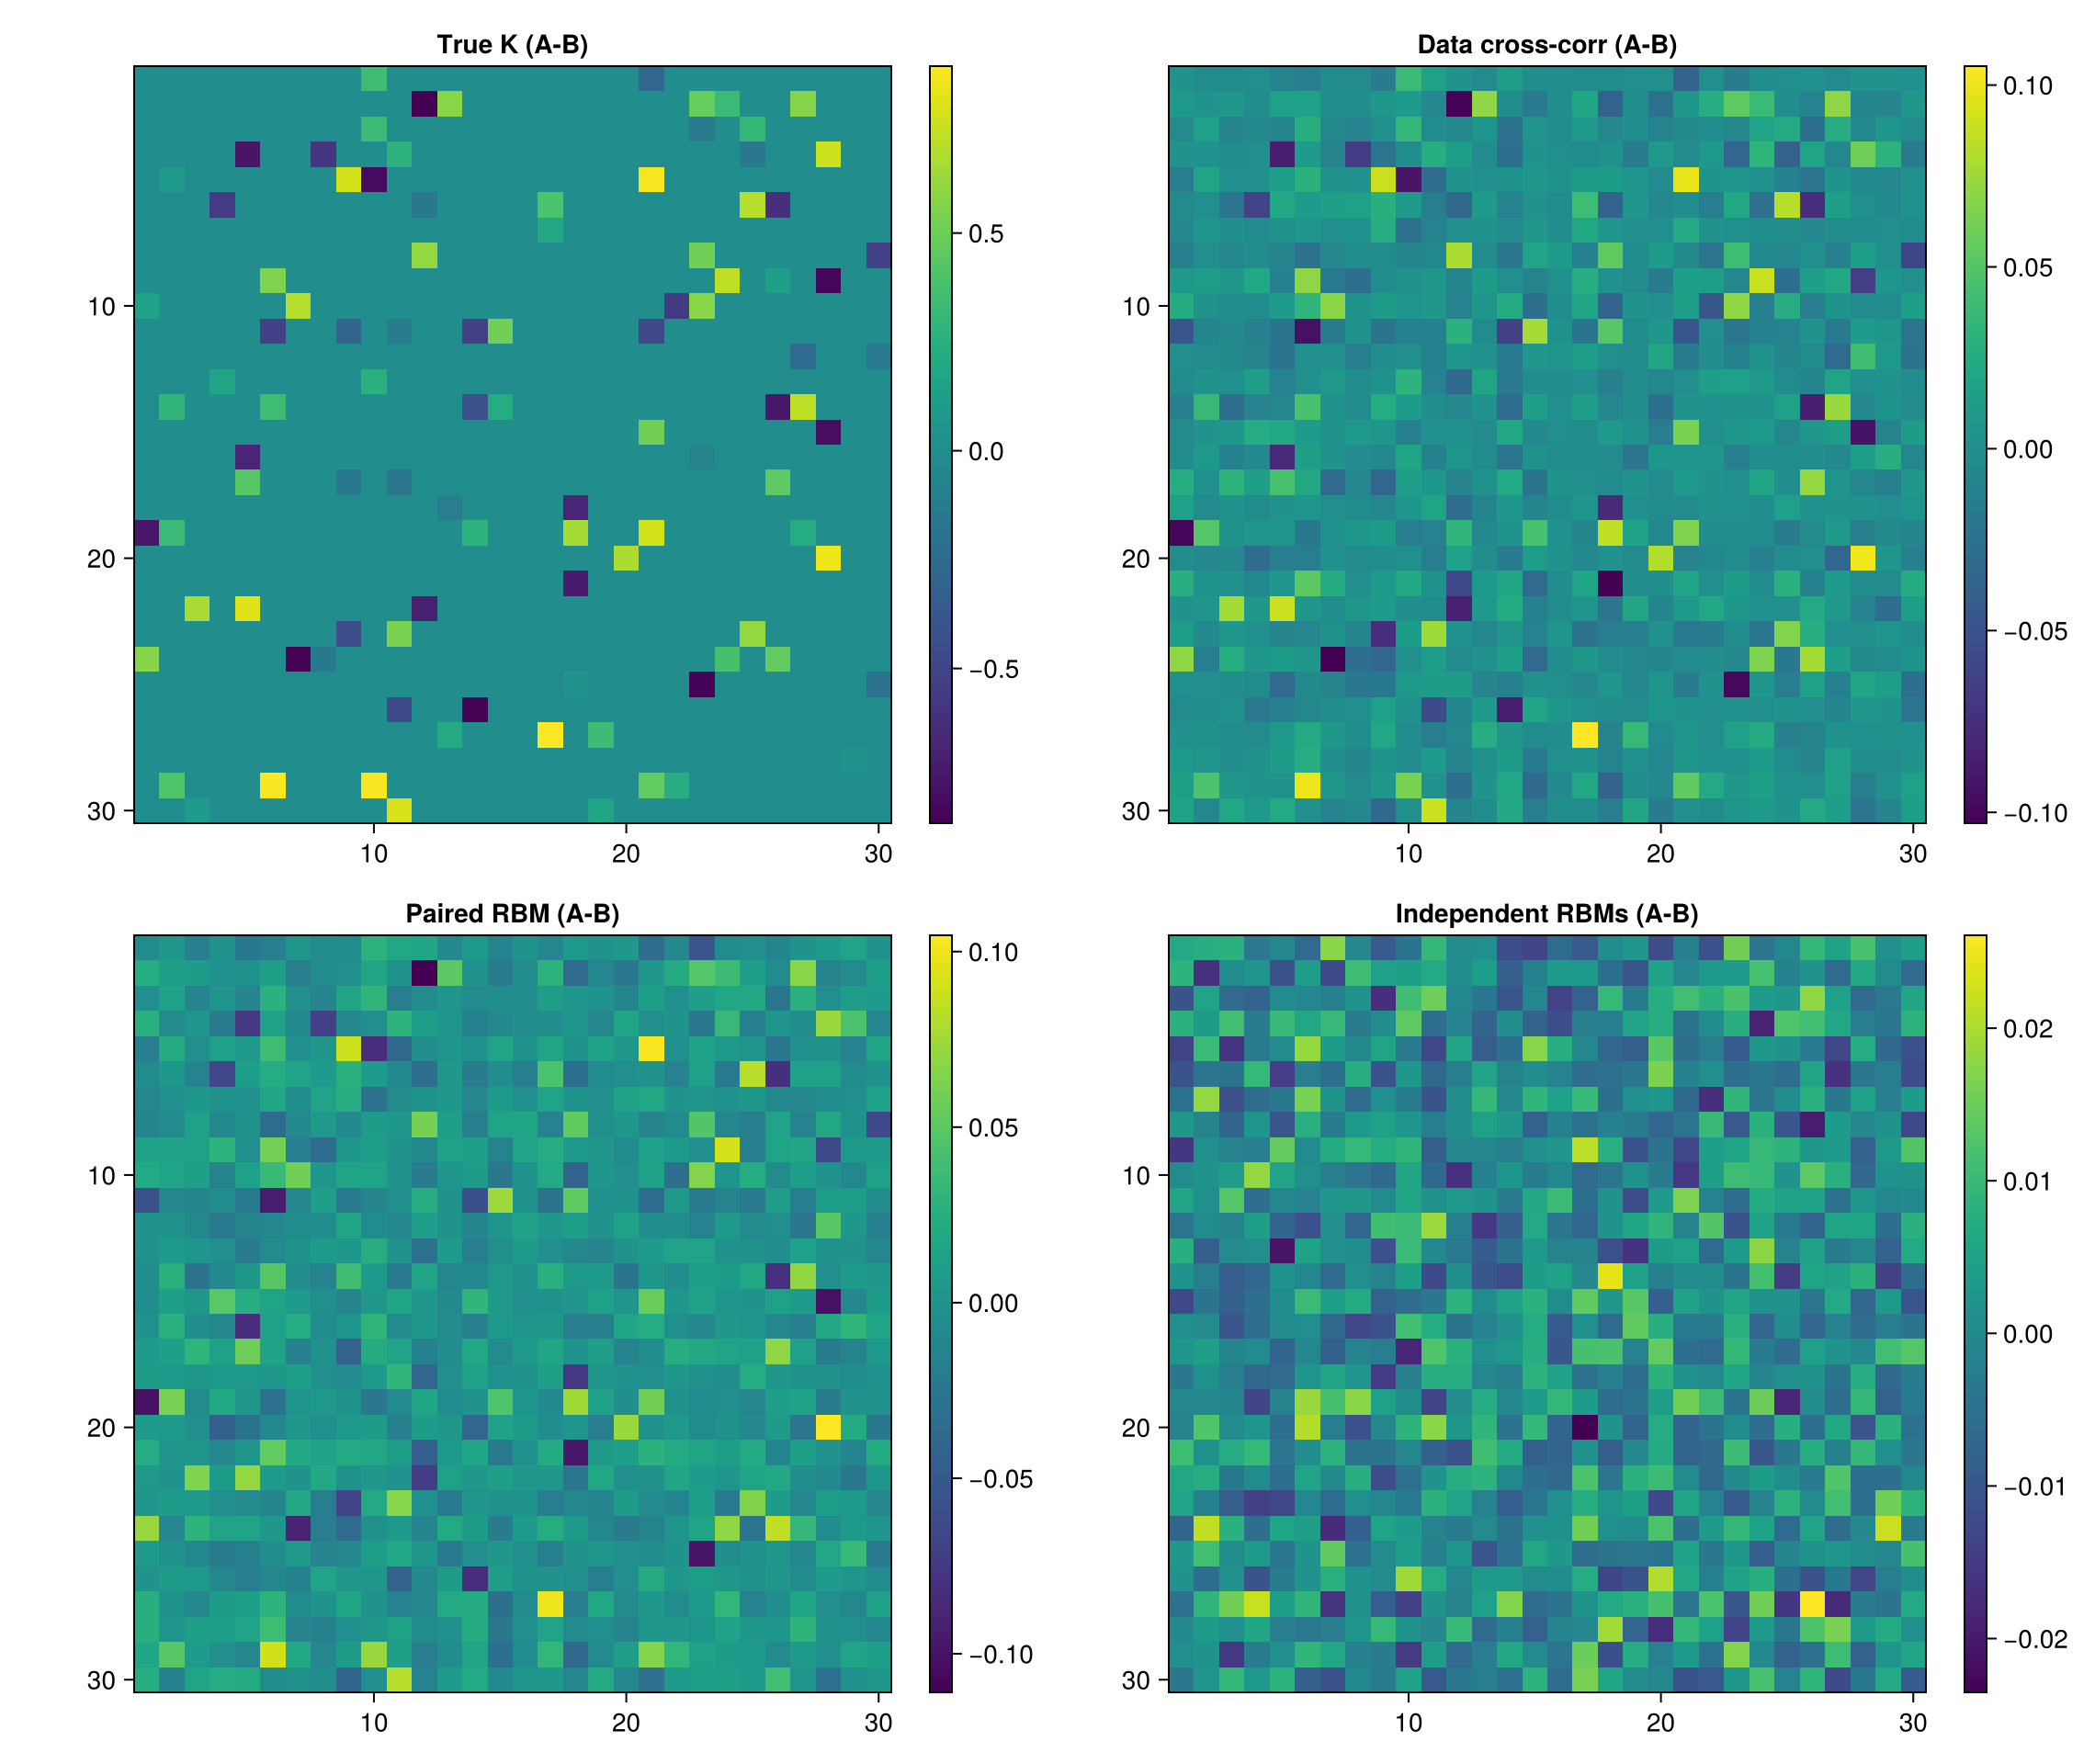
\includegraphics[width=\linewidth]{figures/cross_corr_potts.png}
\caption{Potts + dReLU paired model}
\end{subfigure}
\hfill
\begin{subfigure}[t]{0.48\linewidth}
\centering
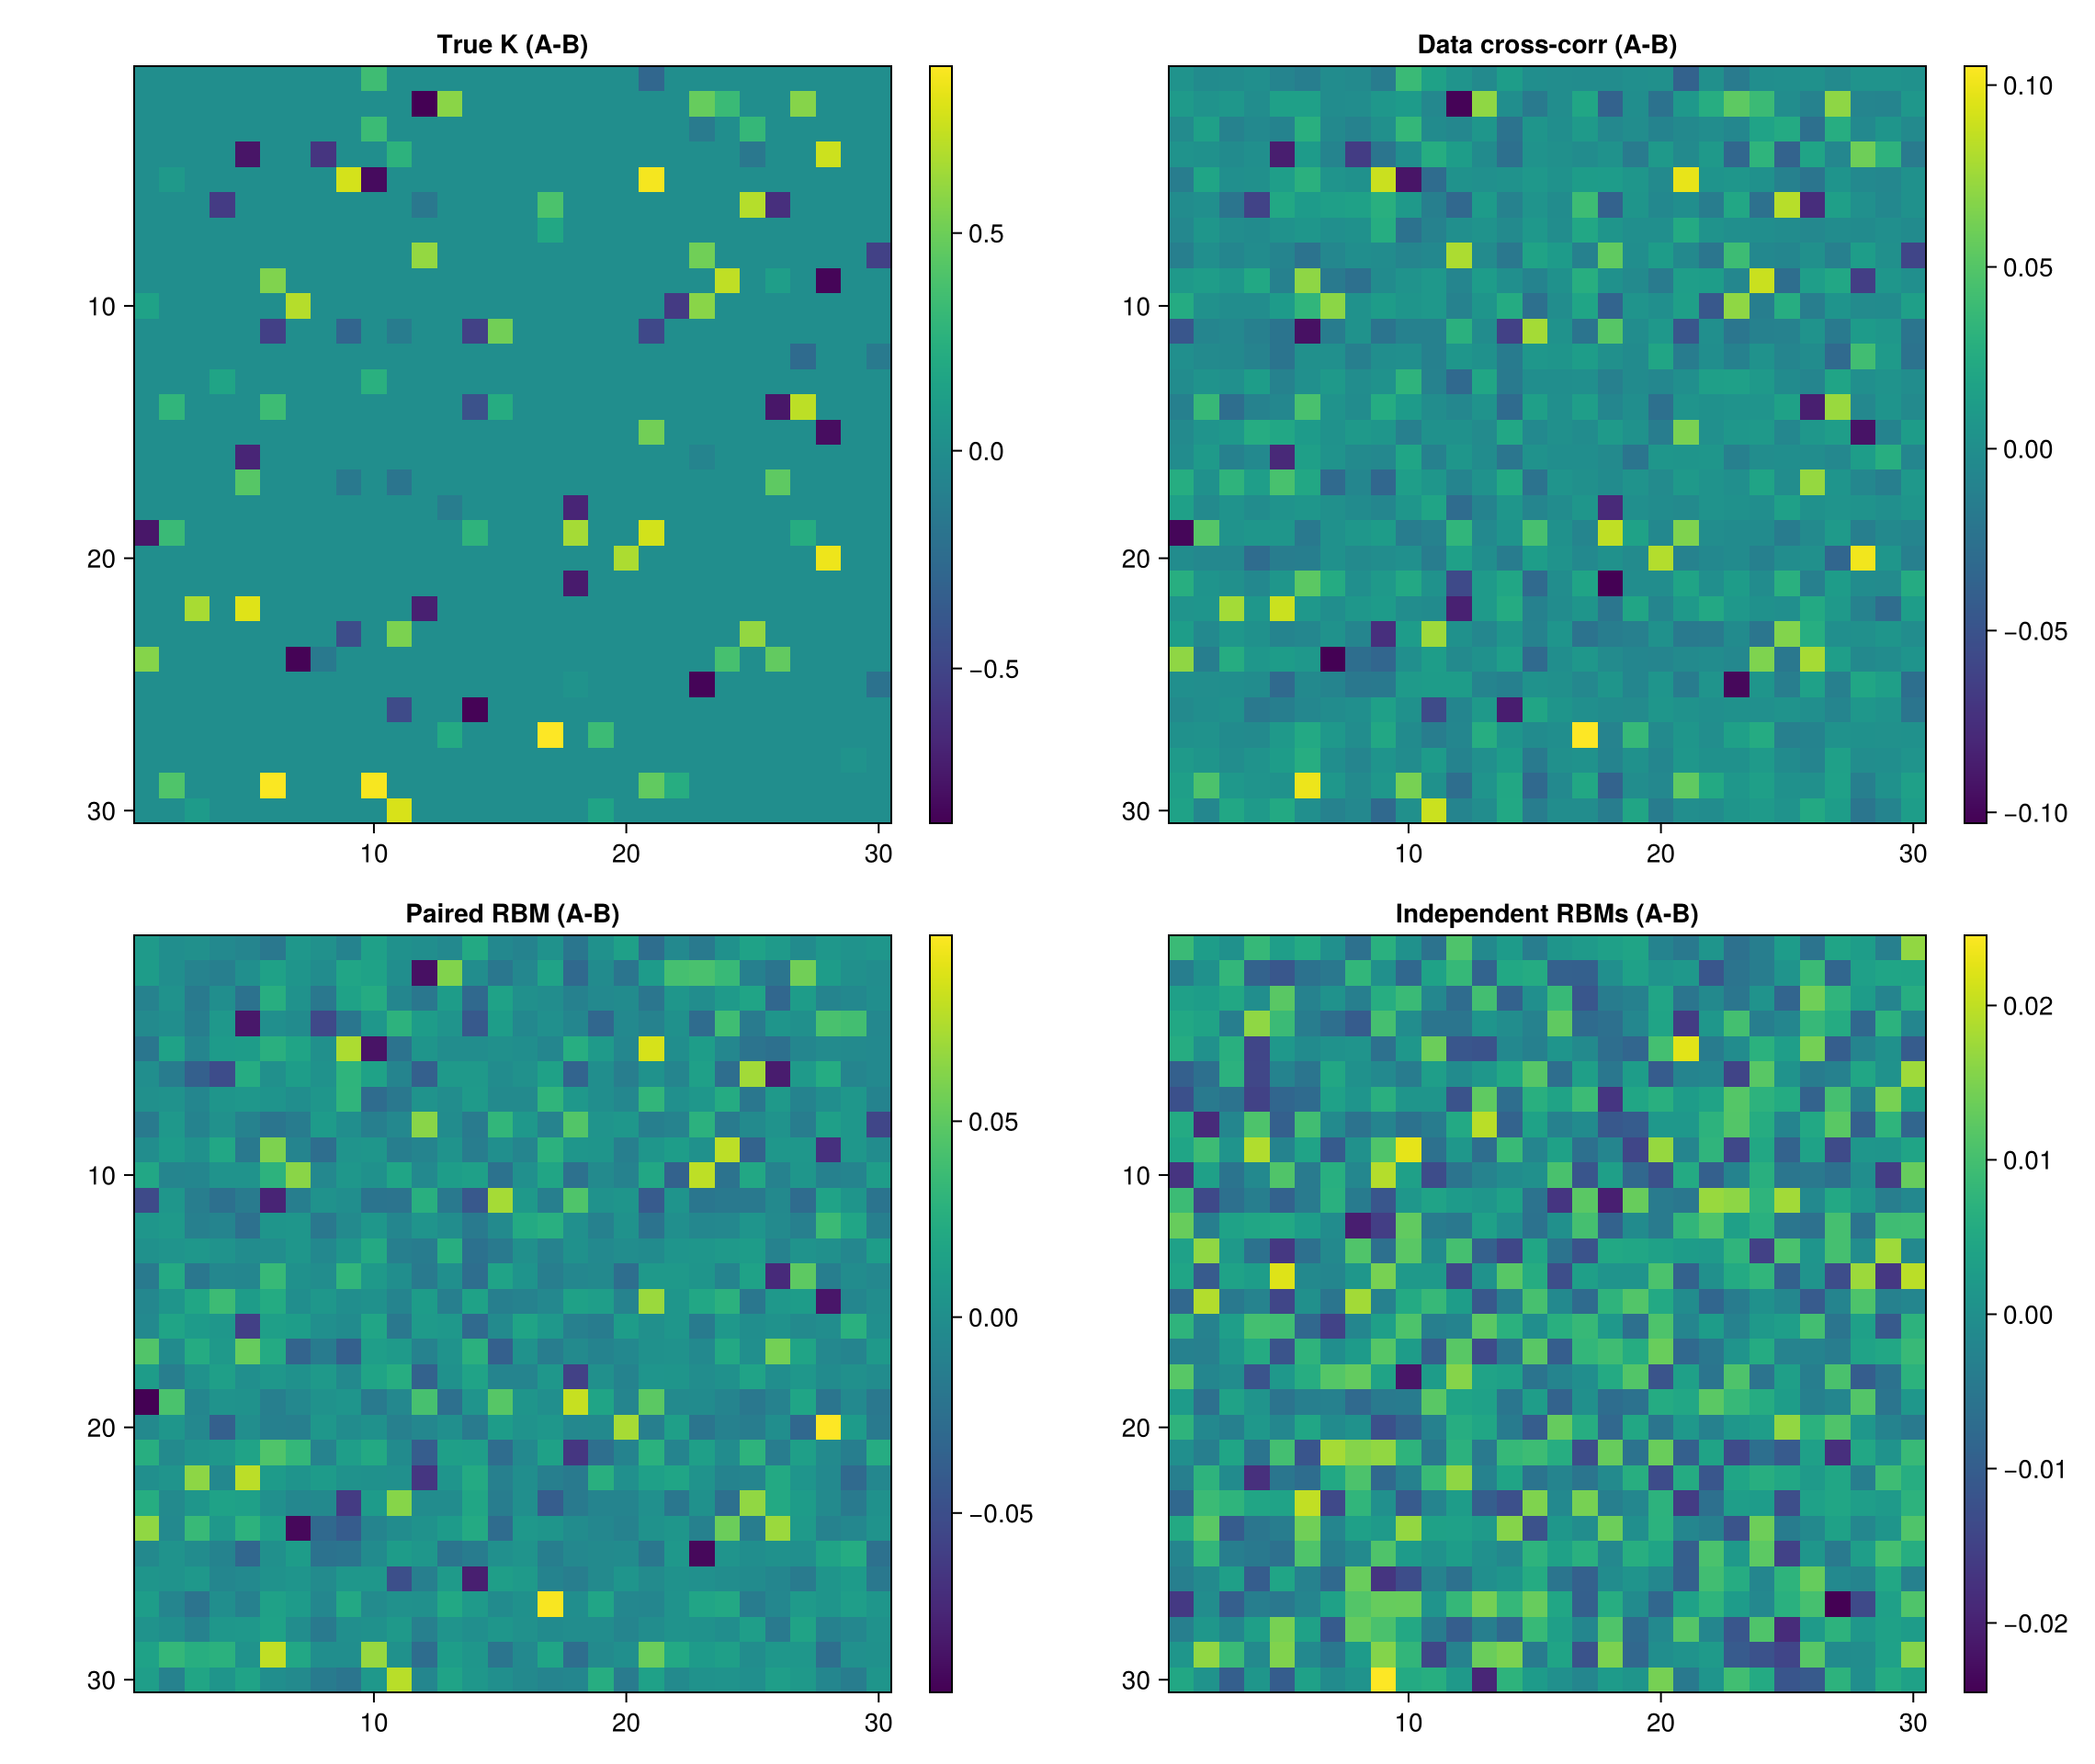
\includegraphics[width=\linewidth]{figures/cross_corr_binary.png}
\caption{Binary paired model}
\end{subfigure}
\caption{Cross-family correlation matrices at equilibrium: true coupling
$K$, empirical training-data correlation, correlation recovered by the
paired model, and correlation obtained from two independent, uncoupled
RBMs. The paired model visibly reproduces the sparse support of $K$ that
is absent from the independent-model baseline.}
\label{fig:crosscorr}
\end{figure}

Finally, recovering cross-family structure does not come at the cost of
corrupting each family's own private statistics
(Fig.~\ref{fig:familypreservation}): residual off-diagonal intra-family
correlation, sampled from the full paired model, stays close to its data
value (family $A$: $0.057\to0.068$; family $B$: $0.048\to0.058$/$0.060$),
a small degradation consistent with weak, indirect intra-family coupling
introduced through the shared hidden layer, not with any breakdown of the
frozen blocks.

\begin{figure}[htb]
\centering
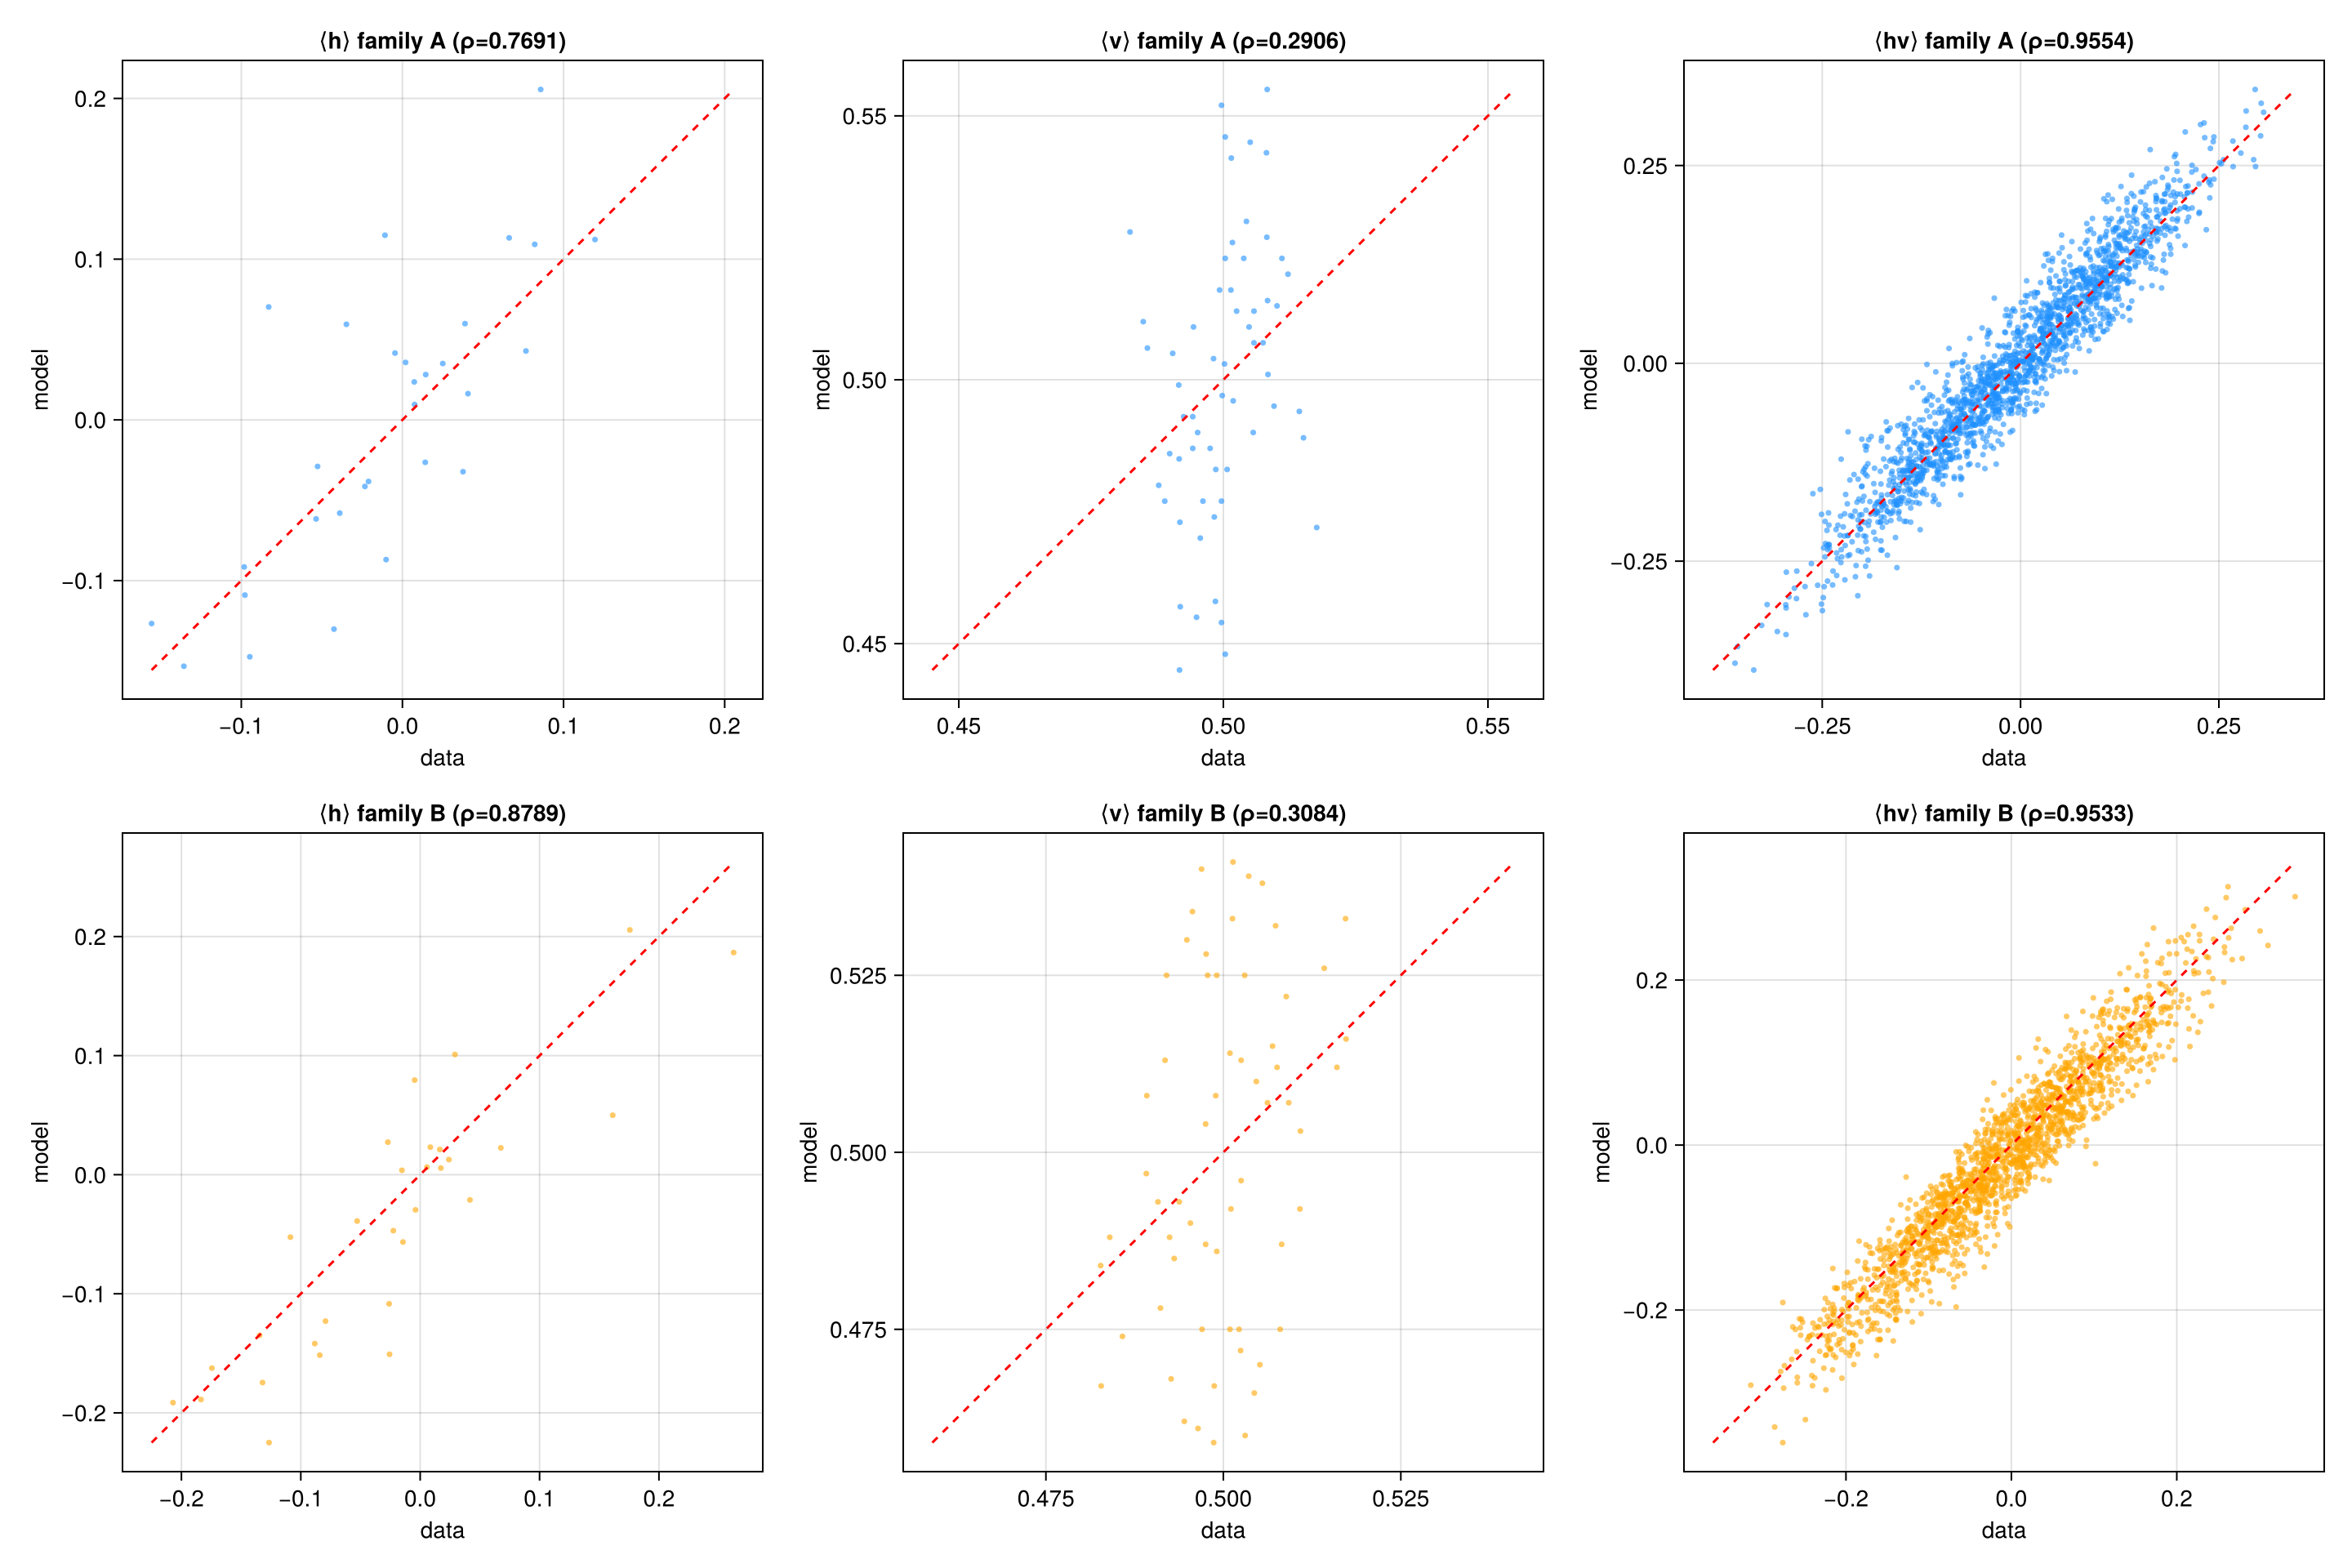
\includegraphics[width=0.62\linewidth]{figures/family_preservation.png}
\caption{Intra-family correlation matrices, data vs.\ paired-model
equilibrium samples, family $A$ and family $B$ separately. The frozen
blocks preserve the private structure learned before pairing, up to a
small perturbation induced by the shared added units.}
\label{fig:familypreservation}
\end{figure}

\subsubsection{Robustness across random seeds}
\label{app:seed}

The result above uses a single realisation of the random intra- and
inter-family couplings and a single training run. To check this is not a
fortunate draw, we repeated the full pretrain--freeze--pair-train
pipeline at three independent random seeds, on the strong-field variant of
the data set (local fields $h\in[-0.3,0.3]$, introduced to keep the
per-site marginal signal well clear of sampling noise) with
$n_{\mathrm{add}}=40$ added units. Table~\ref{tab:seeds} reports the range
across seeds of the same headline quantities as Table~\ref{tab:headline}.

\begin{table}[htb]
\centering
\caption{Equilibrium validation across three random seeds, strong-field
data set, $n_{\mathrm{add}}=40$ ($5000$ Gibbs samples, $5000$ sweeps
burn-in each). Range given as (min--max) across the three seeds.}
\label{tab:seeds}
\begin{tabular}{lccc}
\toprule
 & paired model (range) & data (ceiling) & independent (null, range) \\
\midrule
top-100 overlap & 0.68--0.70 & 0.72 & 0.09--0.12 \\
corr.\ with $K$ & 0.818--0.837 & 0.845 & $-0.04$--$0.05$ \\
\bottomrule
\end{tabular}
\end{table}

The freeze check passes exactly, with zero drift, at every seed; private
RBM pseudolikelihoods and $vh$-correlations ($r\approx0.99$) are likewise
consistent across seeds. The spread across seeds is small relative to the
gap between the paired model and the null, confirming that the qualitative
recovery reported above is a stable property of the construction in this
setting, not an artefact of one particular random draw.

\subsubsection{Potts versus Binary}

The Potts+dReLU variant performs modestly but consistently better than
the Binary RBM on training-time diagnostics (private-model $vh$-correlation
$0.94$ vs.\ $0.87$; added-unit equilibrium tracking $\rho=0.997$ vs.\
$0.81$), yet this advantage barely shows up in the decisive test against
ground truth (top-$K$ overlap $0.67$ vs.\ $0.65$; correlation with $K$
$0.796$ vs.\ $0.786$). The categorical representation appears to yield
cleaner internal statistics, without materially changing how much genuine
cross-family signal is ultimately extracted in this regime.

\subsection{Discussion}

A small, dedicated block of hidden units, added on top of two frozen,
independently pretrained models, recovers the large majority of an
otherwise hidden inter-family coupling structure, confirmed directly
against known ground truth by equilibrium Monte Carlo sampling rather
than inferred indirectly from training curves. Two caveats: the density
of the inter-family coupling matters (the sparser, $n_{\mathrm{links}}=20$
data set still clears the independent-model baseline, but with a
noticeably weaker absolute signal, indicating very sparse, weak
cross-couplings are harder to disentangle from sampling noise at fixed
training length); and the natural whole-matrix correlation against a
sparse ground truth carries a structural ceiling well below $1$
(Section~\ref{sec:sparsity}), making the finite-sample ceiling, not
$r=1$, the correct benchmark throughout.

This remains a controlled, minimal test bed, validated at its headline
configuration and, separately, confirmed stable across three random seeds
at a second configuration (Section~\ref{app:seed}); a systematic scan of
$\beta$, hidden-layer size, or training length was not performed. A
natural next step, orthogonal to the real-data question of
Section~\ref{sec:protein}, is a systematic scan over $n_{\mathrm{add}}$
and over inter-family coupling density and strength, extending the
single-configuration headline result and the seed-robustness check into a
full map of where the freeze-and-add construction stops being sufficient
and a fuller joint retraining becomes necessary.

\end{document}
